\taughtsession{Lecture}{Border Gateway Protocol}{2023-11-23}{0900}{Thanos}{}

\section{Introduction}
Border Gateway Protocol (BGP) was developed in 1989. It is a path vector exterior gateway protocol which operates on the core layer of the network. This means it is not contained within autonomous systems, rather it connects autonomous systems together. BGP is used as an inter-domain routing solution, which connects Internet Service Providers together, such as BT, Virgin, Sky, etc. The current implementation of BGP (BGP4) was initially ratified as RFC 1771 in 1994, which includes Classless Inter-Domain Routing (CIDR). 

\section{Characteristics of BGP}
BGP uses a composite metric, operates on the exterior of the network and is a path vector protocol. It is a singlepath protocol which uses multicast to send updates. It operates in a hierarchical structure with the current version including classless support. BGP is highly configurable, much more than RIP or OSPF - this can introduce security issues from misconfiguration. BGP is modular which means it can be made to work the way that you want it to operate. 

\section{Using BGP}
\subsection{When to Use BGP?}
With BGP being an inter-autonomous system routing protocol, it is predominantly used by ISPs who facilitate inter-autonomous system routing. This allows companies to connect to the ISP and use default routing to forward the packet to another autonomous system, without having to worry about how it gets there. However - some companies do actually use BGP, especially if they utilise more than one ISP; using BGP allows them to configure redundant links for auto-failover (where they would loose connection to one ISP and automatically start using the second ISP).\\

BGP operates on \textit{edge routers} which sit on the extremeties of autonomous systems. Packets are forwarded from edge router to edge router by BGP, and when the packet arrives at the destination network - OSPF or RIP is used to get the packet to the right device. 
\subsection{Uses of BGP}
Some multi-national organisations use BGP to tie their geographically separated locations together. This process is called \textit{peering} and would then allow the multiple Autonomous Systems to behave as though its one single system. OSPF would also be able to achieve this, which would mitigate the need for BGP. BGP is a complex routing algorithm and as such it should not be used where there is a \textit{viable} alternative. 

\section{How BGP Works}
\begin{figure}[ht]
    \centering
    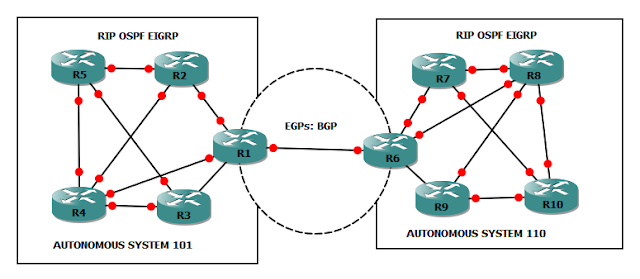
\includegraphics[width=0.9\textwidth]{assets/bgp-implementation.png}
    \caption{Diagram showing where BGP operates between two Autonomous Systems}
    \label{fig:bgp-implementation}
\end{figure}

Figure \ref{fig:bgp-implementation} shows how two autonomous systems can be connected together using BGP. The diagram also shows how autonomous systems have a unique numerical identifier.\\

BGP is a \textit{path vector} routing protocol, this means it advertises paths not links however it doesn't use distance vector methods similar to what RIP does. BGP uses the full path to the destination by maintaining a list of autonomous systems that packets must pass through to reach the target network. BGP uses a number of attributes to learn each route, the use of which allows routing policies to be implemented.\\ 

\textit{Routing Policies} allow control over what routing prefixes are distributed between interconnected ISPs and between ISPs and their customers. This allows BGP to be \textit{deterministic}. This means that an administrator has granular control over what routes are accepted or rejected. This is controlled by setting of a preference of one route over another to a particular network. All of this determinism is underpinned by routing policies, hence these are key to inter-domain routing.\\

Many ISPs create and enforce \textit{Service Level Agreements} (SLAs) through routing policies. This gives them the ability to control exactly who, what and how much traffic can be transmitted through their network for any given period of time. It is not uncommon for a policy file to be multiple thousand lines long in a backbone ISP.\\

It is the ability to shape traffic through path attributes that is the fundamental difference between BGP and interior routing protocols.

\subsection{BGP Peer Sessions}
BGP operates on BGP enabled routers which form relationships with other BGP enabled routers. Each route has a \textit{Network Layer Reachability Information} (NLRI) value. This is composed of the IP prefix ID and length along with attributes for the route. A BGP router may have a peer relationship with one or more BGP speaking routers. 

\subsection{BGP Router Discovery}
In BGP routing - neighbours are not discovered automatically as in other protocols, rather each pair of BGP speakers that will exchange routing information must be configured manually. This is implemented by design as it means peer relationships are only established between organisations doing business with one another.

\subsection{BGP Sessions [beyond the specification]}
Peer sessions between BGP speakers commence with the opening of a TCP connection between the routers, BGP relies on this for reliable communication. The TCP session is opened on Port 179. Upon initialising of a TCP session, a pair of BGP speakers exchange the entire contents of their \textit{Adj-RIBs-Out Database}. After that, only updates are sent and only when the contents of the Adj-RIBs-Out changes, which is known as triggered updates. The TCP session stays open with keep-alive packets, which means that if the session is terminated - the initialisation process starts again. 

\subsection{BGP Path Determination [beyond the specification]}
BGP does not incorporate the traditional metrics of interior routing protocols. Instead, paths are chosen for use through Routing Policies. BGP stores all learned routes and their attributes in \textit{Adj-RIB-In} which is raw, unprocessed routing data. Routes to be installed and / or advertised go through a three-part decision process. 
\begin{enumerate}
    \item Calculate the degree of preference for each route in Adj-RIB-In
    \begin{itemize}
        \item Internal Peer: the degree of preference is calculated based on policy information or calculated on the \verb|LOCAL_PREF| attribute
        \item External Peer: the degree of preference is strictly based on policy information
    \end{itemize}
    \item Install the best route to each destination into Loc-RIB
    \begin{itemize}
        \item Each feasible route is first checked to see if the net hop router specified in the \verb|NEXT_HOP| attribute is reachable
        \item If the \verb|NEXT_HOP| is not reachable, the route is dropped
        \item Then the \verb|AS-PATH| variable is checked to be sure the route is not looped
        \item Qualifying routes are then installed to Loc-RIB based on the following criteria: if only one route is available, it is installed; whereas if there are multiple routes to the same destination - install the route with the highest degree of preference as calculated in step 1.
        \item If there are multiple routes to the same destination with the same preference value, a set of tie-breaking rules are engaged
    \end{itemize}
    Tie-break: The algorithm iterates through a series of steps that eliminate routes, the algorithm terminates when only one route remains.
    \item Route Dissemination
    \begin{itemize}
        \item Select which routes in Loc-RIB will be advertised
        \item This selection process is based on configured routing policy
        \item Any configured route aggregation also takes place here. 
    \end{itemize}
\end{enumerate}

\section{Autonomous Systems}
An \textit{Autonomous System} (AS) is defined as a collection of networks under common Administrative Control. A single organisation can be considered an AS. An AS is not determined by any size considerations, rather it provides a common administrative control while sharing a routing strategy. It is the network responsible of any given AS who takes responsibility of using a suitable routing strategy, that encompasses all the networks attributed to the AS.\\

It is expected that the users of External Gateway Protocols are usually ISPs, these wil include more than one organisation and therefore more than one Autonomous System. In this case - the ISP is responsible for routing to and from their customers \& any transit traffic passing through to other ASs.

\subsection{Autonomous System Numbering}
In a similar fashion to the Internet Protocol using IP addresses for identification, ASs used in BGP also need to be identified. This is accomplished through assigning each AS a unique \textit{Autonomous System Number} (ASN). The \textit{Internet Assigned Numbers Authority} (IANA) is the global authority who is responsible for coordinating the ASNs.\\

The American ASN authority is \textit{ARIN}, who use 16-bit numbers ranging from 1 to 65535. Their public ASN space is 1 to 64511, with every AS connecting to the core of the internet must have a public ASN. The range 64512 to 65535 are designated as private ASNs. These are utilised for functions such as private peering between two ISPs, however are never used on the public internet. Obviously, 65535 is not enough ASNs; a review is currently underway to extend these to 32-bit numbers. 

